\documentclass[openany]{book}
\usepackage[utf8]{inputenc}
\usepackage{graphicx}
\usepackage[a4paper, total={6in, 8in}]{geometry}
\renewcommand{\baselinestretch}{1.3}

\title{Learning Depth and Visual Odometry From Light Fields \\
\large AMME4111 Thesis A Progress Report}

\author{Joseph Daniel}
\date{November 2019}

\begin{document}

\maketitle

\tableofcontents

\chapter{Introduction}
Humans have a remarkable ability to perceive visual stimuli emanating from the world around them. Not only do we identify different objects, scene depth, movement, and colour with ease, but we often draw meaning and even enjoyment from the combination of light rays bouncing around space and arriving at our eyes. We are able to automatically compensate for differences in lighting and viewing angle, and we can extract complex information such as emotion from what we process visually. To word it concisely, the human visual perception system is one of the most versatile and robust image processing machines that we know of. Most man-made machines on the other hand are much more easily decomposed into a set of deterministic modules that require explicit, well defined instruction sets. Often, when given an image, there is no straightforward function that directly maps from pixel intensities to the semantic meaning of that image. As researchers tackling problems in computer vision, we are usually interested in developing the algorithms that can help machines not only sense the world, but perceive it in a way that is useful. The objective of this thesis project is to develop a pipeline that simultaneously learns to perform two tasks. The first is visual odometry - the act of estimating camera motion from a sequence of images. The growth of autonomous robotics has meant that there is an ever-growing need for accurate navigation and localisation when satellite positioning is unavailable or wheel encoder odometry is unreliable. An autonomous unmanned aerial vehicle navigating an unknown indoor environment is one example where visual odometry is a valuable feedback signal that can be used to precisely control the UAV's position. The second is depth estimation, that is, discerning the distance of objects in a scene from the imaging device. The ability to perform depth estimation from visual cues is desirable in applications such as autonomous vehicles where navigating new environments whilst avoiding collisions is a basic requirement. Being able to draw depth information from a camera sensor will help to enable these capabilities, especially in applications where methods such as Lidar or RGBD sensors are prohibitive - small quad-copters and internal medical imaging devices are examples where this might be the case.


Humans are exceptionally well adapted to these tasks - our two eyes allow us to process the 3D geometry of the scene, while our learned experiences are often able to fill in the gaps where geometric information is insufficient or unavailable. Unfortunately, image processing algorithms are not equipped with this same kind of human intuition, and so the deceptively complex task of estimating the 3D structure of a scene from a sequence of images continues to attract attention from the computer vision community. 


The price of camera components is decreasing while image quality continues to improve, not only making cameras an attractive perception module for autonomous robotics, but also spurring the popularity of multiple-view imaging. Embracing this idea, this thesis project seeks to develop a pipeline that performs these tasks by taking advantage of the rich geometric information exposed when using multiple views. Thus, this thesis project adopts the vocabulary and the concepts from the area of light field imaging. The light field describes the intensities and directions of each light ray in space, providing a convenient way of thinking about multi-view geometry which is embraced throughout this thesis.


Another core objective of this thesis is to develop a pipeline that relies principally on unsupervised machine learning models to perform the two tasks side-by-side. This approach is chosen with the intention that a data-driven model can build a robustness to scenarios that are difficult to design for using hand crafted solutions.  Furthermore, this pipeline will benefit from being self-supervised - unlike data-driven models that require direct supervision from labelled data to improve their performance (classifying images of cats and dogs is a common example), this pipeline has no intermediary requirements between the data collection and training routines. Not only does this mean that the expensive process of hand-labelling data is unnecessary for this pipeline to function, but the model will be able to continue learning, benefiting from new data collected in situ. An adaptive perception module that learns to operate effectively in new environments is a desirable capability in robotics, especially when considering that effects such as thermal expansion, vibration and shocks can frequently render our equipment calibrations meaningless in the field. 

In this progress report we will first establish the conceptual groundwork that this thesis builds upon with a discussion surrounding the seminal texts that have shaped the state-of-the-art literature in visual odometry and depth estimation. In understanding those texts, we demonstrate that existing methods have yielded excellent results, whilst identifying that there is a substantial potential for improvement on state-of-the-art results using multi-view imaging devices. 


\chapter{Literature Survey}

\section{Machine Learning in Computer Vision}

An oft-quoted anecdote in computer vision tells of MIT researcher Seymour Papert, who in 1966 assigned a summer project that sounded simple enough, namely to construct a 'visual system' that could describe what objects it saw by name \cite{papert1966vision}. While the regimes of computer vision have evolved substantially since 1966, many of the ideas, and challenges have persisted. This is embodied in the popularity of projects such as the ImageNet Large Scale Visual Recognition Challenge (ILSVRC) \cite{ilsvrc}, drawing researchers from institutions around the world. It was at the ILSVRC annual challenge where in 2012, a convolutional neural network achieved a top-5 error rate of 15.3\%, outperforming all previous submissions by 10.8\% \cite{krizhevsky2012alexnet}. Until 'AlexNet' in 2012, the competition subsisted of competitors introducing algorithms that produced marginal improvements year on year. Needless to say, an improvement of over 10\% made a big splash in computer vision, drawing attention to the powerful capabilities of deep learning.

While deep neural networks for computer vision have gained massive popularity since the success of AlexNet, the history of neural architecture models begins much earlier, with the perceptron as described by Frank Rosenblatt in \cite{rosenblatt1959neurodynamics}. The fundamental building block of neural networks, the 'perceptron' is a module that accepts several inputs, and produces a single output computed as a weighted sum of each input - allowing complex functions to be approximated when several perceptrons are layered together as a 'multilayer perceptron' \cite{minsky1969perceptrons}. The process of finding the optimal set of weights that produce the desired output given a set of inputs is referred to as training, and in practice is usually found by optimising some cost function using the backpropagation algorithm \cite{rumelhart1986backprop}. 

Convolutional neural networks (CNN's) are similar to multilayer perceptrons, but introduce a spatial invariance that makes them particularly well suited for extracting high-level features from image data. Where multilayer perceptrons are densely connected, the connectivity pattern of each node in a CNN takes advantage of the hierarchical organisation of patterns in image data by using a 'receptive field'. Biologically inspired, these nodes respond to stimuli only in their receptive field, and so they typically learn to identify salient 'features' in the image - combinations of pixels that represent some kind of underlying structure. As these types of networks grow deeper, the features that they learn typically become more complex \cite{lecun1989cnn}. Early layers are provided with a small region of the image, typically a window between 3 and 11 pixels wide, and so will usually learn quite primitive features such as lines and corners. Deeper layers however may learn to recognise higher-level features such as eyes and mouths, and eventually even human and animal faces.

\begin{figure}[tbp]
    \centering
    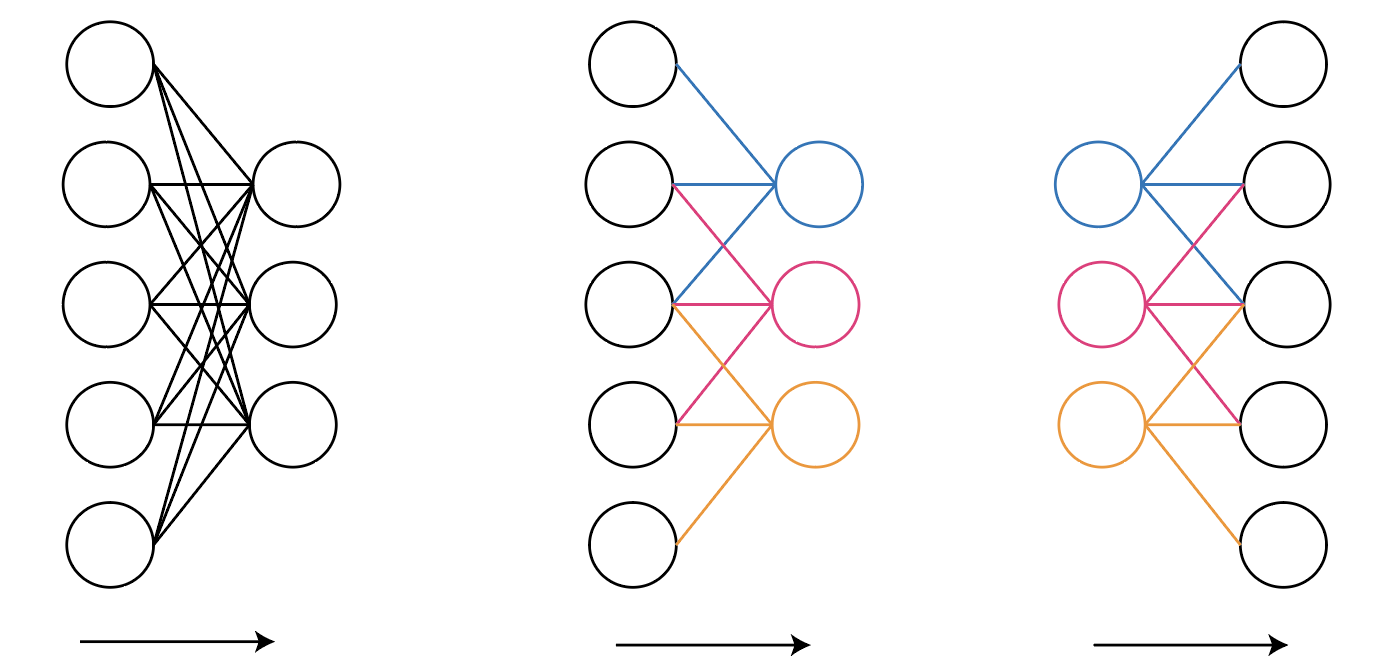
\includegraphics[width=5in]{images/cnnvsmlp.png}
    
    \caption{Multilayer Perceptron (left): each output from one layer is fed into the inputs of every node in the subsequent layer. Convolutional Neural Networks (middle) on the other hand have a 'receptive field', taking advantage of the spatial coherence of pixels in image data. The convolutional upsampling operation (right) is frequently used to upsample a low-dimensional feature space, to a higher dimensional one. It is often employed as a 'learned' information decompression.}
    
    \label{convexhull}
\end{figure}

CNN's are thus popular 'feature extractors' in computer vision - their ability to learn to respond to different types of stimuli mean that they have been used as a dimensionality downsampling tool, taking the millions of dimensions present in digital images  and compressing them to a feature space with a much smaller number of parameters. Closely related is the convolutional upsampling operation which performs the inverse - taking a feature space and learning to upsample that feature space into something meaningful \cite{long2014fcn}. This has given rise to a particular topology of CNN called the encoder-decoder architecture, which will be useful throughout this thesis. The encoder part of a CNN is composed of a series of convolutional down sampling operations - this can be thought of as finding an efficient compression of the information stored in the image. The decoder subsequently uses this compressed form of the information to extract some meaningful information about it. One example where this architecture has been used is in \cite{long2014fcn}, which outputs a classification for each pixel in the image. In this thesis, a fully convolutional encoder-decoder architecture will be used for a similar purpose, but rather than classifying each pixel into one of several categories, it will regress depth values for each pixel. 


\section{Depth Estimation and Visual Odometry}

Since the invention of the pinhole camera, most cameras have captured 2D representations of a 3D world, meaning information about physical structure is lost. With the addition of a second viewpoint however we can learn a little more about the shape of the scene as governed by epipolar geometry \cite{zisserman2004multiview}. Meanwhile, a video is a sequence of images, taken in very quick succession, and so one could think of video footage as a multi-view camera where each image is separated not only spatially but also temporally. Identifying the amount of motion between two temporal frames of the video camera is the goal of visual odometry, where one intuitive approach is to observe the direction of movement of each pixel between the pair of images. In practice, features such as SURF \cite{bay2008surf} or SIFT \cite{lowe2004sift} features are used to simplify the search for image correspondences. The essential matrix, which describes the relationship between two cameras in space can then be estimated using techniques such as the 5 or 8 point algorithm. 

\subsection{The Monocular Approach}
Doing so monocularly however is problematic because with a single camera there is no way of concretely discerning the actual magnitude of the movement based on pixel data alone, meaning some kind of scale factor needs to be estimated based on characteristics of the image \cite{gakne2018scale, nister2004vo, zhou2016scale, zhou2019scale}. In fact, this scale ambiguity is often exploited by film makers - what appears as a sweeping shot of a vast landscape on the big screen is often modeled as a miniature film set in the studio. Because the image is monocular, there is no way to ground our measurements of scale in real world units, and so we resort to our imaginations and learned experiences to fill in the gaps. What \textit{is} preserved in these monocular setups however is the overall structure of the scene and motion of the camera - we may not know how large the object is or how far the camera has moved, but we \textit{can} compute the  shape of the object as well as the direction of camera motion. 

\subsection{The Stereo Approach}


\subsection{The Plenoptic Flow Approach}


\subsection{The Machine Learning Approach}

One recent approach that has driven a large body of research is the use machine learning to perform both of these tasks, utilising convolutional neural networks to learn a non-linear mapping directly from a pair of images to their depth maps, as well as the relative pose between them \cite{eigen2014supervised, garg2016unsupervised,godard2016consistency, liu2015supervised, zhou2017unsupervised}. Combining the spatial awareness of the convolutional down sampling operation with a neural networks ability to learn accurate approximations for complex, non linear functions, these approaches have found success in both supervised \cite{liu2015supervised, eigen2014supervised}, and unsupervised settings \cite{garg2016unsupervised, godard2016consistency, zhou2017unsupervised}. In the supervised family of algorithms, \cite{eigen2014supervised} and \cite{liu2015supervised} take advantage of datasets such as KITTI \cite{dataset-kitti}, containing ground truth depth maps collected using state-of-the-art depth sensors and poses measured from inertial sensors. 

Unsupervised experiments such as \cite{garg2016unsupervised, godard2016consistency,zhou2017unsupervised} on the other hand exploit the constraints imposed by epipolar geometry to learn depth either by using known camera poses or by estimating pose in addition to depth. The general pipeline utilises two CNN's, one who's purpose is to predict dense per-pixel depth maps given a single image, and the other who's job is to estimate the 6 degree-of-freedom pose from the first frame to the second given both images.

\begin{figure}[htbp]
    \centering
    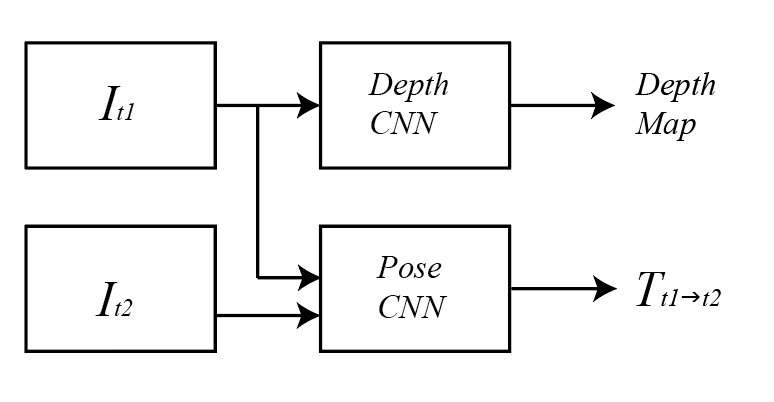
\includegraphics[width=3in]{images/cnns.png}
    \caption{Machine learning approaches have demonstrated strong results in simultaneously estimating depth maps and relative poses between images. Typically, a pair of CNN's is used, one for each task. The depth CNN is provided with the first view at $t=1$ and the pose CNN is provided both views.}
    \label{2cnns}
\end{figure}


While the training pipeline is unsupervised in the sense that labelled data is not required, some form of supervision signal is nevertheless required to optimise the parameters of the pair of networks. These papers take advantage of the fact that if the physical structure of a scene is known, then a novel rendering of that scene from a different viewpoint is achievable. Thus, \cite{garg2016unsupervised} suggested using photometric reconstruction as a supervision signal - from $I_{t2}$, reconstruct $I_{t1}$. The difference between the reconstruction and the real image can form a supervisory signal for the pair of networks. 


\begin{equation}
    L_{photometric} = \sum_m^W \sum_n^H |I_{t1}(m,n) - \hat{I_{t1}}(m,n)|
\end{equation}


Humans can easily imagine what a scene will look like if we move our heads slightly, but only if we know the overall shape of the object we are looking at. Similarly, given two images separated by a small interval of time $I_{t1}$ and $I_{t2}$, one could synthesise what $I_{t1}$ would look like by sampling the pixels from $I_{t2}$, if the relative pose $T_{t1\rightarrow t2}$ between the two cameras and a pixel-wise depth of the scene $D_{t1}(p)$ is known. In practice, this can be done by obtaining the projected coordinates of $p_{t1}$ on $I_{t2}$'s camera sensor. Assuming a pinhole model, the complete expression for $p_{t1}$'s projected location on the second camera, $\hat{p_{t2}}$ is 

\begin{equation}
\hat{p_{t2}} = KT_{t1\rightarrow t2} D(p_{t1}) K^{-1} p_{t1}
\end{equation}

where K represents the intrinsics matrix. The obtained coordinate $\hat{p_{t2}}$ is continuous, while pixel coordinates are discrete. A pixel value thus needs to be interpolated, keeping in mind that each step of a neural network pipeline must be differentiable to support the backpropagation of gradients. 

\cite{zhou2017unsupervised} suggested adopting the use of bilinear sampling as a fully differentiable sampling mechanism, as first proposed in \cite{jaderberg2015spatialtransformer}. A bilinear sampling kernel is described by 

\begin{equation}
    V = \sum_n^H \sum_m^W U_{nm} max (0, 1-|x - m|) max(0, 1-|y - n|)
\end{equation}

Where $V$ is the output of the sampling kernel, $U$ is the source image being sampled, $n$ and $m$ index over the columns and rows of the kernel respectively, $H$ and $W$ are the height and width of the sampling kernel, and $x$ and $y$ are the local coordinates of the sampling location. The equation is differentiable with respect to x and y:


\begin{equation}
    \frac{\partial{V}}{\partial{x}} = \sum_n^H \sum_m^W U_{nm} max(0, 1-|y - n|)
\end{equation}
\begin{equation}
    \frac{\partial{V}}{\partial{y}} = \sum_n^H \sum_m^W U_{nm} max(0, 1-|x - m|)
\end{equation}

Using this bilinear sampling kernel, we can thus sample pixels from $I_{t2}$ to reconstruct $I_{t1}$ in a fully differentiable manner, allowing the backpropagation of gradients through the networks. The pipeline with photometric reconstruction as the supervision signal can be illustrated as: 


\begin{figure}
    \centering 
    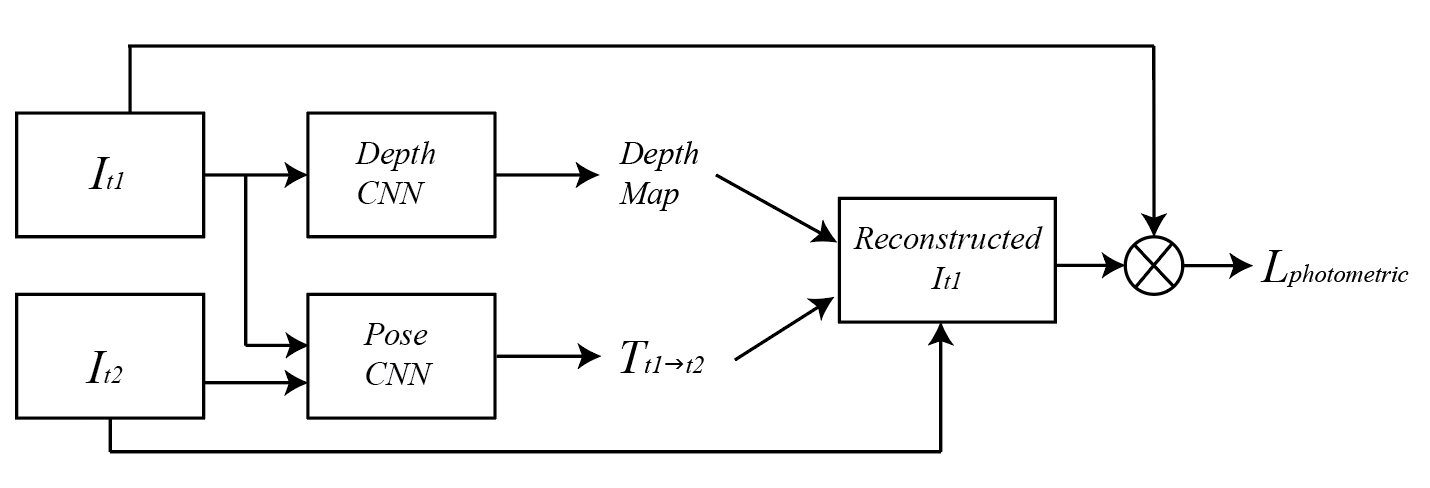
\includegraphics[width=5in]{images/mlpipeline.png}
\end{figure}

\section{The Light Field and Multiple View Geometry}

Light field imaging has emerged as a powerful tool in computer vision for robotics, offering a rich higher-dimensional representation than what can be captured by conventional optics. The underlying principle used to describe the light field is the plenoptic function, a 7-dimensional mapping that assigns radiance values to the light rays at every position in space, in every orientation, at all wavelengths, throughout all of time \cite{ihrke2016lfprinciples}. \cite{adelson1991plenoptic} shows that this can be formally expressed as $L(x,y,z,\theta, \phi, \lambda, t)$, and measured in $W/m^2/sr/nm/s$. 
With the addition of practical constraints however, the plenoptic function can be expressed more concisely as a parameterisation of 4 variables. 

Pixels on camera sensors integrate the number of photons arriving at them over a finite period of time removing the temporal dimension, and each colour channel can be thought of as a monochromatic sampling of the light field, removing the spectral dimension. Additionally, and importantly, is the constraint that the radiance of light rays propagating through a vacuum do not change if samples are restricted to the convex hull of the scene, thus reducing the overall dimensionality of the plenoptic function by one parameter \cite{levoy1996lfrendering}. To illustrate this, one could think of the light rays leaving the inside of a bowl sat upright on a table. Many of those rays may only travel a small distance before being blocked by the inside of the bowl itself, meaning those rays will never be registered by any practical measurement device. As shown in figure \ref{convexhull} if we consider only the convex hull of the bowl however, we are required only to represent the value of the plenoptic function on the encapsulating surface of the object \cite{gortler1996lumigraph}.

\begin{figure}[htbp]
    \centering
    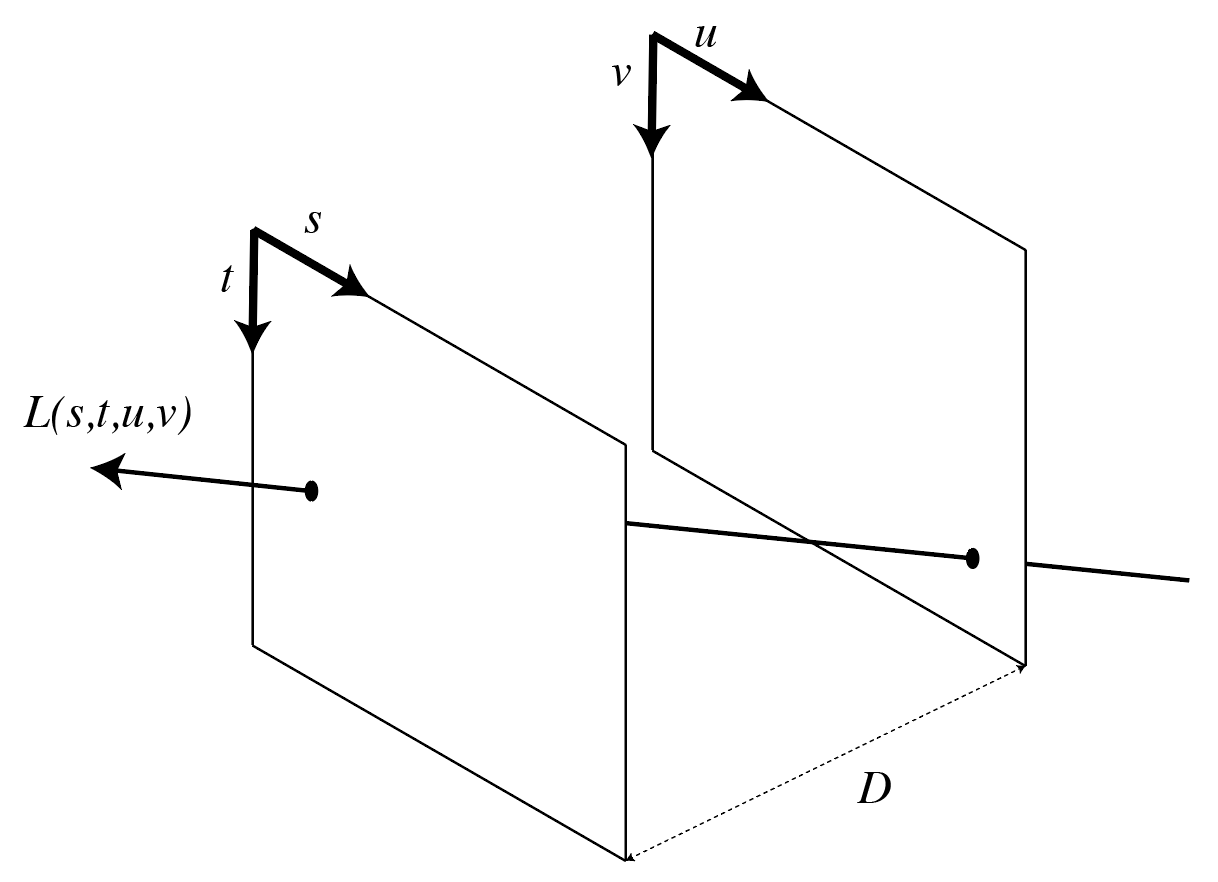
\includegraphics[width=2.5in]{images/2pp.png}
    
\includegraphics[width=0.3in]{images/blank.png}
    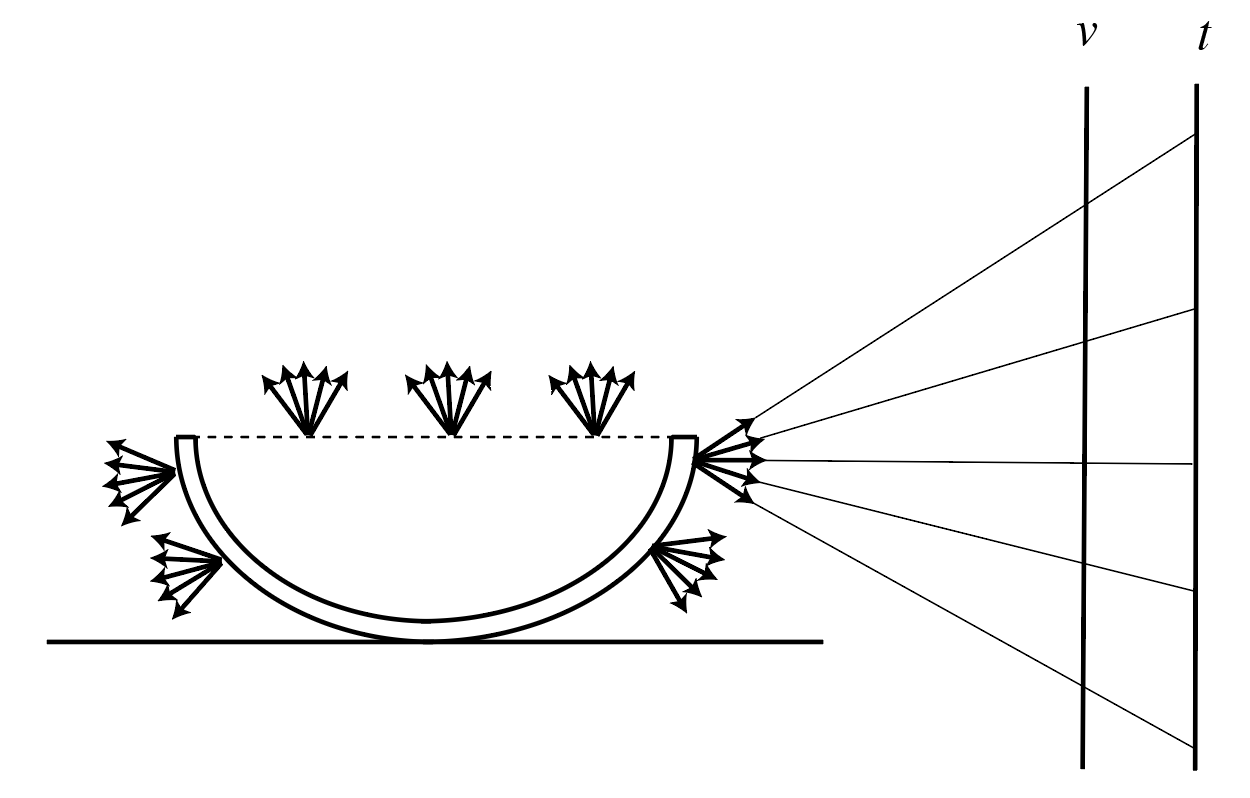
\includegraphics[width=2.5in]{images/convexhull.png}
    
    \caption{Two plane parameterisation (left): the plenoptic function can be described by the radiance along a ray passing through two parallel planes. The free space assumption (right): if we consider only the bundle of rays leaving from the convex hull of the object at a particular instance in time, in a single colour channel, we can parameterise the light rays as a function of 4 variables rather than 7.}
    
    \label{convexhull}
\end{figure}

Also illustrated is a common convention for describing light rays in this 4 dimensional space called the two plane parameterisation. In this parameterisation, two parallel planes are used to fix both the position and orientation of each ray by fixing their points of intersection with two parallel planes. By convention, the plane closest to the scene it termed \textit{u, v} and the plane closest to the camera sensor is the \textit{s, t} plane.



This 4D realisation of the light field originated as a model of rendering 3D computer graphics, one which shifted emphasis from notions of texture and geometric primitives to modeling the behaviour of light rays permeating space. Since then however, the conceptual framework of the light field has drawn a following of researchers at an intersecting region of signal processing, computer vision and robotics \cite{dansereau2014phd}. This notion of light field imaging finds a foothold in this thesis project through the utilisation of camera arrays, which are devices that sample multiple views of the same scene. Using a camera array is a simple method for acquiring a dense sample of the light field, where the position of the camera determines \textit{(s,t)} while the location of the pixel determines \textit{(u, v)} \cite{yao2016camarray}. The images captured from a camera array are mapped easily to the 4D light field, and identifying corresponding pixels across images exposes a rich tapestry of geometric information about the scene. 


\begin{figure}[tbp]
    \centering
    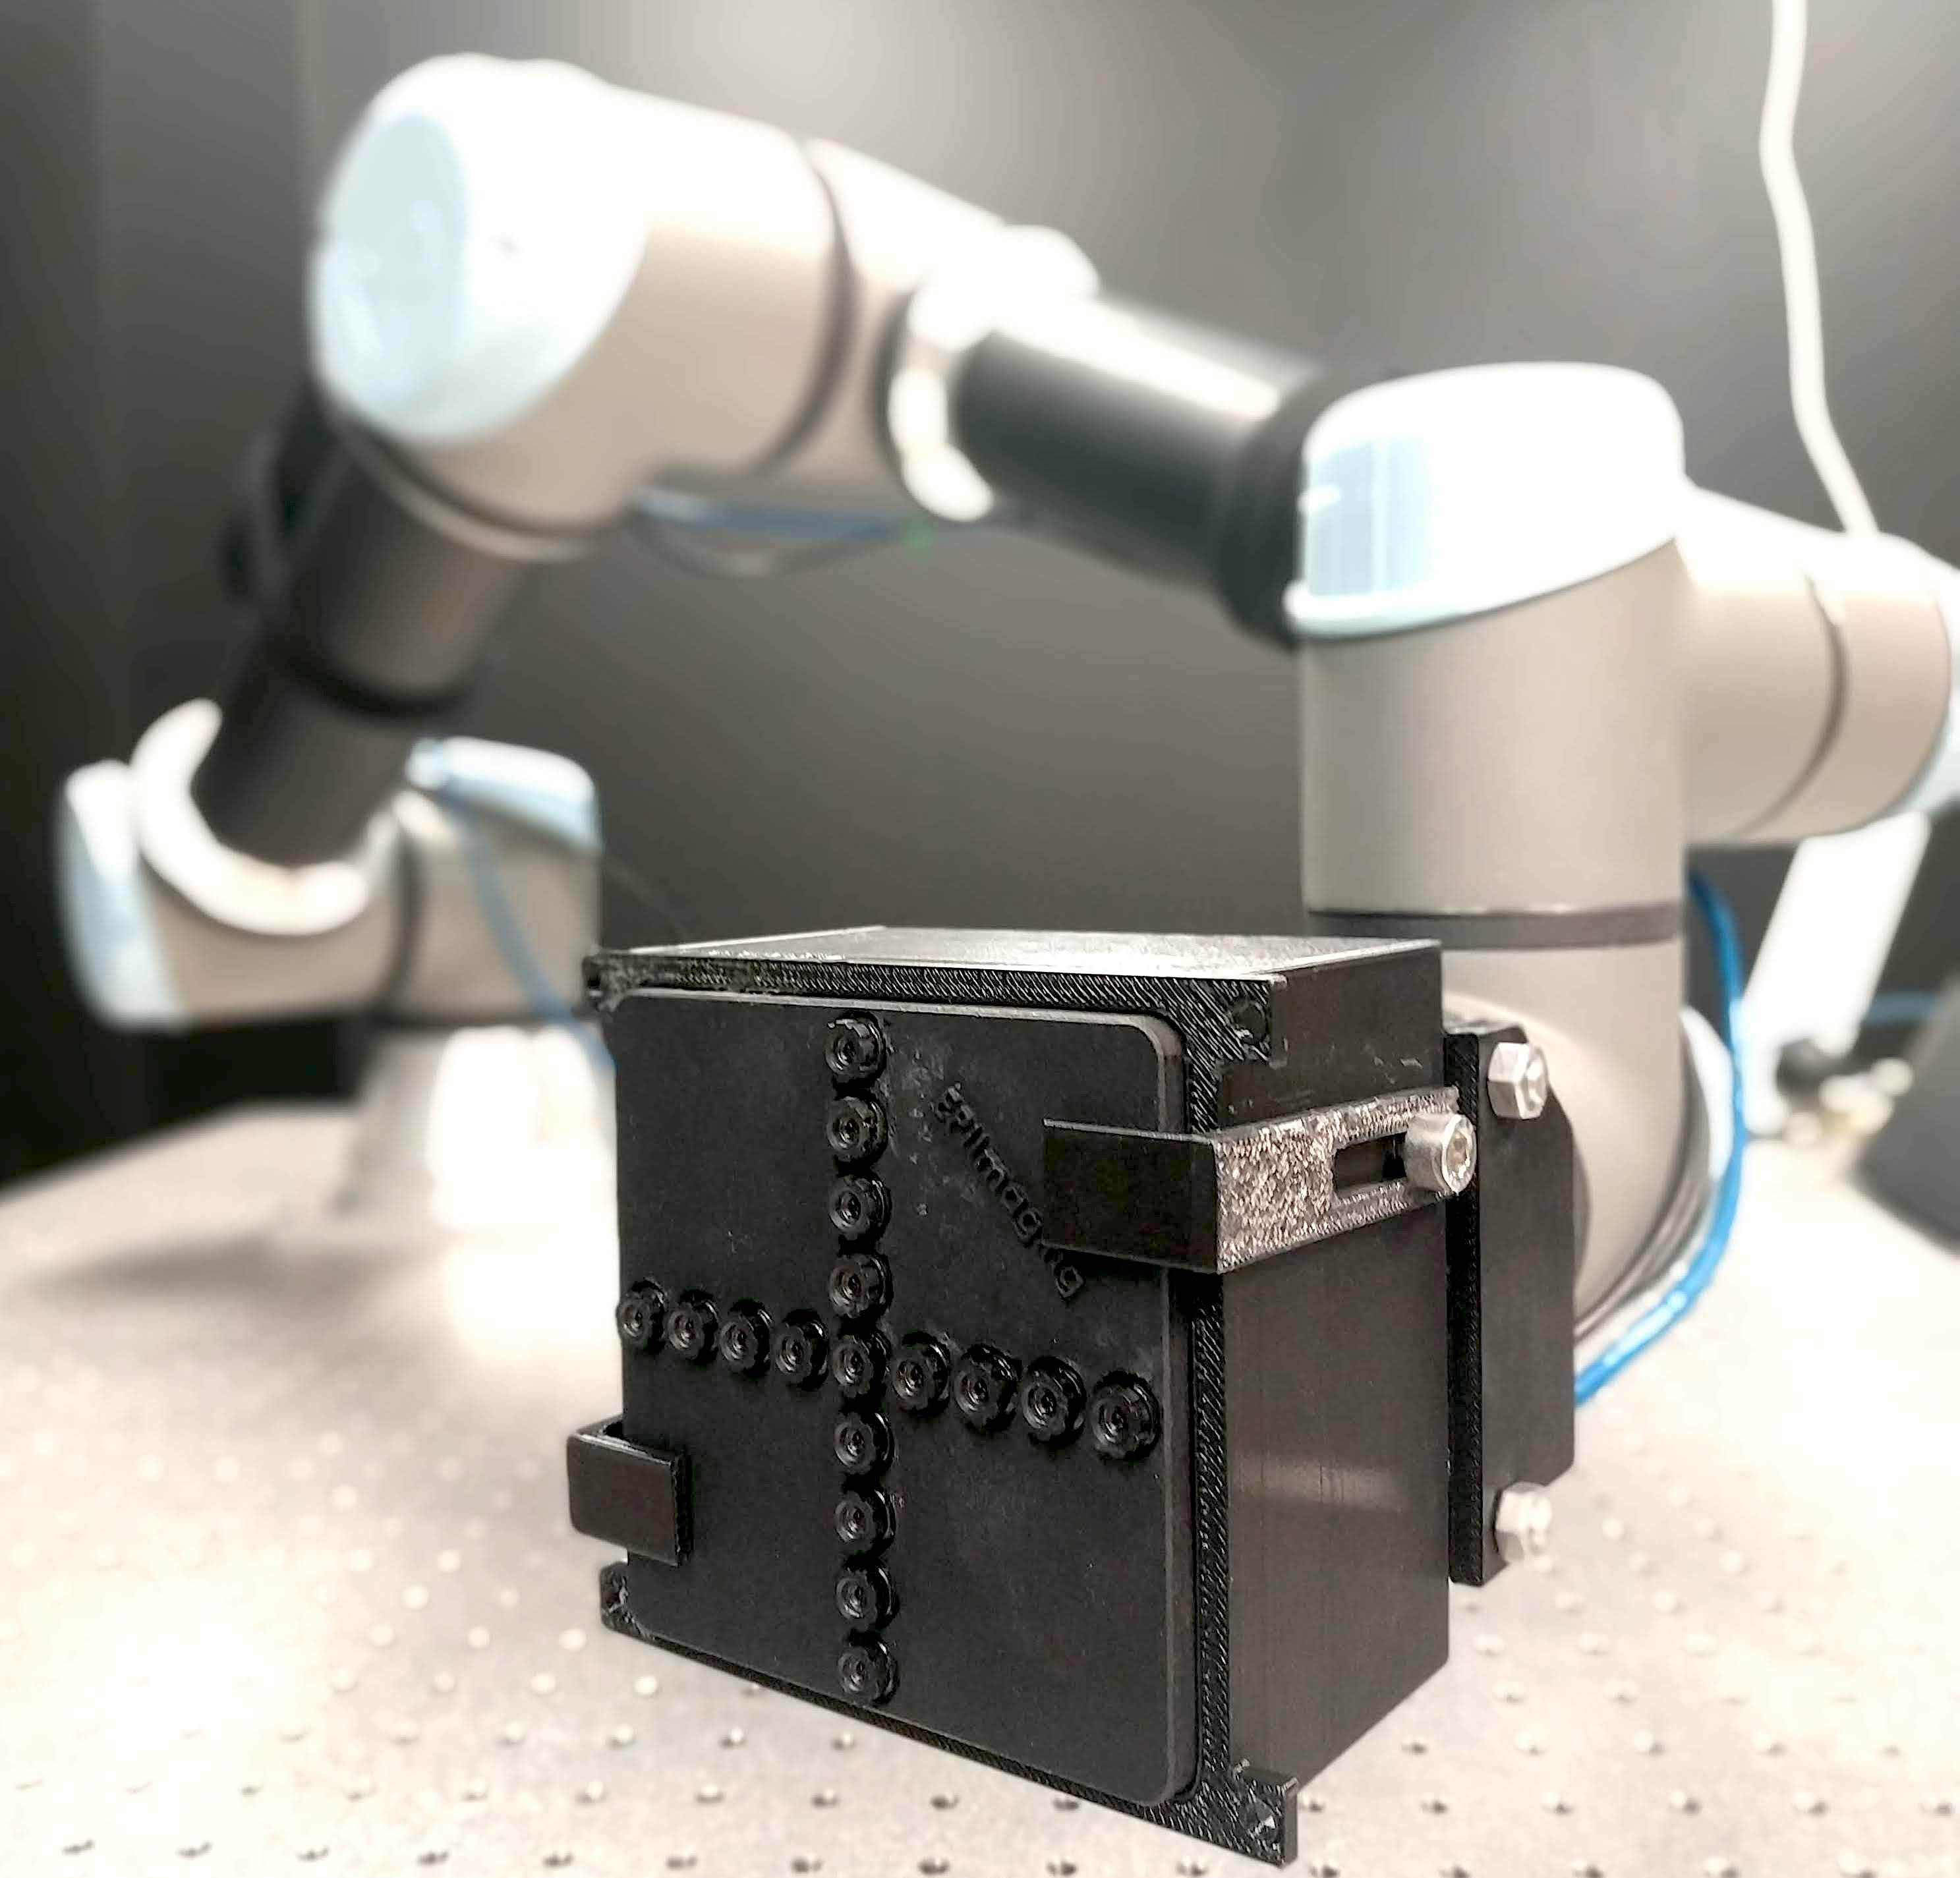
\includegraphics[width=4.5in]{images/robotcamera.jpg}
    \caption{An example of a camera array mounted on a robotic arm. This camera array is configured as 17 sub-apertures arranged on a single plane in a cross-hair formation. Camera arrays sample several views of the same scene and are thus capable of acquiring a dense sample of the light field.}
    \label{cameraarray}
    \vspace{1cm}
    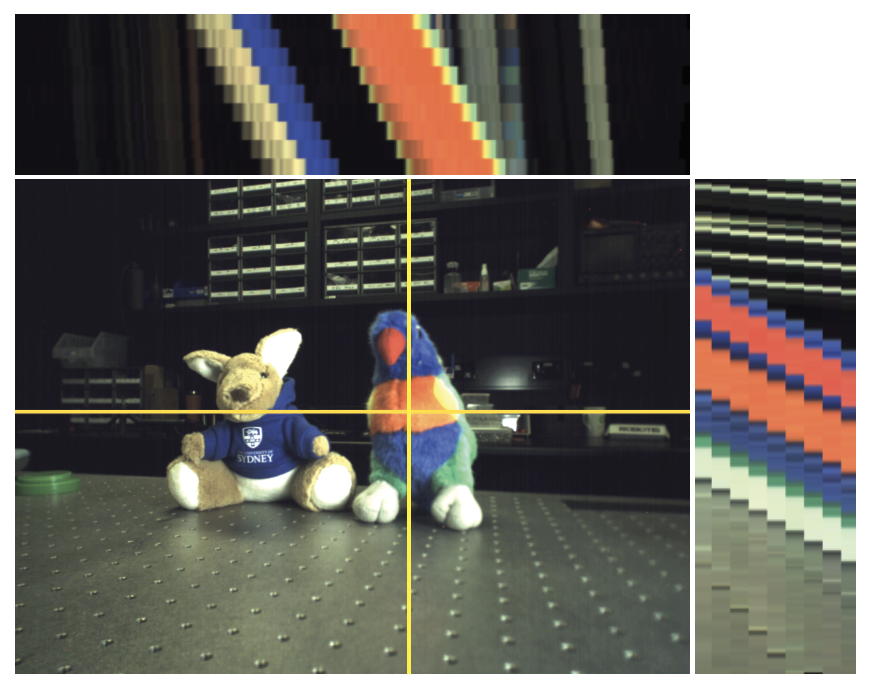
\includegraphics[width=1.6in]{images/epipolarimage.png}
    
\includegraphics[width=0.4in]{images/blank.png}
    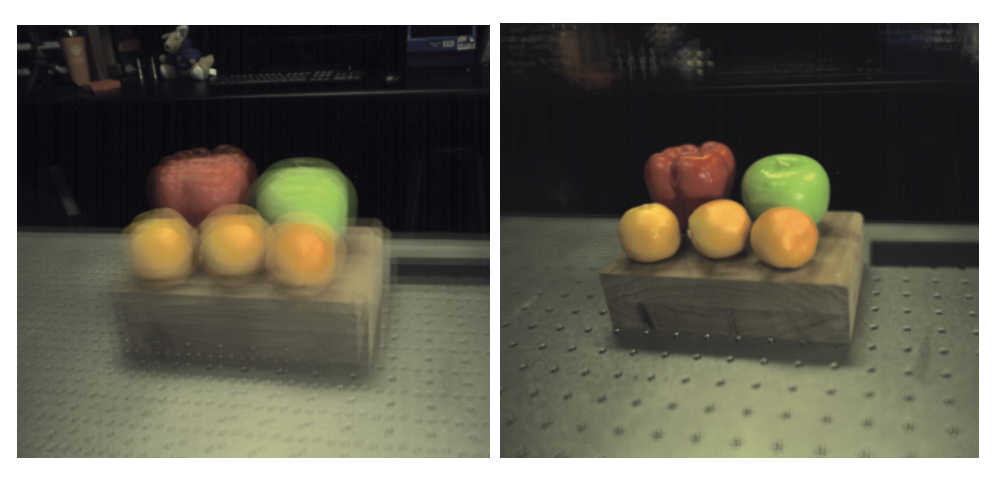
\includegraphics[width=3.5in]{images/fruitfocus.png}
    \caption{Epipolar Plane Images (left): Shown as a slice of a volume, the images formed by dissecting the image in the \textit{s,u} and \textit{t,v} planes are characterised by sheared straight lines, with the grade of the slope encoding the amount of parallax experienced by a pixel at that \textit{u} or \textit{v} coordinate. Synthetic aperture focusing (right): taking the average of every image from the camera array yields an image where different parts are in focus depending on the alignments of the images.}
    \label{epiplaneimg}
\end{figure}


One way that this geometric information can be easily visualised is by taking slices of the light field image in the \textit{s,u} or \textit{t, v} axes as shown in figure \ref{epiplaneimg}. While the idea of taking a 2D slice from the 4D image can seem complex, the task of generating a so called 'epipolar plane image' from a camera array is deceptively simple. Images captured from camera arrays can be stacked to form a solid volume, from which 2D slices can be sampled. Each of these slices yields an image characterised by sheared straight lines, encoding information about the geometry of the scene, including depth and occlusions \cite{bolles1987epiplane}. 

The geometric information encoded in a light field sampling can alternatively be visualised by processing the image into a 'focal stack'. Focal stacks closely resemble images with shallow depth of field such as those that can be captured from a commercial DSLR camera. Light field focal stacks differ from focus in the optical sense however in that they are synthetic and can be recomputed after the image has been taken, effectively allowing control over the depth of field and focal depth in post-processing. Focal stacks can be computed from camera array images by layering images over one another and taking the average value for each pixel. The result is that parts of the scene that closely overlap appear in focus while areas with poor overlap create a 'bokeh' effect. More formally, if the relative pose of each camera is known, a specific focal stack for any desired depth can be computed by projecting each image onto the desired focal plane, and computing their average \cite{vaish2004parallax}.

These representations of the light field will play an important role in this thesis project as we experiment with different methods for feeding light field images to the machine learning pipeline. An important consideration in any machine learning algorithm is the feature space - based on what particular inputs will the algorithm be making its decision? Raw images contain millions of measurements and thus represent an incredibly high-dimensional feature space for neural networks to process. Light field images are several times larger, and thus it is important that some form of dimensionality reduction is used to ease the training process. With the goal of investigating effective methods of feeding light fields to neural networks, this thesis will explore the use of three different light field formats as the entry point to the machine learning pipeline. The first two will be the focal stack, and epipolar plane image described above, interpreting the images as a 3 dimensional volume created by stacking 2 dimensional images on top of one another. The third will treat the light field as a 4 dimensional volume, requiring a 3D signal processing pipeline to fully take advantage of the dimensionality.


\chapter{Progress Report}

\chapter{Updated Research Proposal}


\newpage

%\newpage
\bibliographystyle{plain}
\bibliography{bibliography.bib}

\end{document}
